\documentclass[11pt,a4paper]{article}

% ── Packages ──────────────────────────────────────────────────────────────
\usepackage[utf8]{inputenc}
\usepackage[T1]{fontenc}
\usepackage[margin=2.5cm]{geometry}
\usepackage{amsmath,amssymb,amsfonts}
\usepackage{graphicx}
\usepackage[numbers,sort&compress]{natbib}
\usepackage{hyperref}
\usepackage{enumitem}
\usepackage{booktabs}
\usepackage{xcolor}
\usepackage{tikz}
\usetikzlibrary{positioning}
\usepackage{caption}
\usepackage{subcaption}
\usepackage{float}
\usepackage{multirow}
\usepackage{array}

\hypersetup{
    colorlinks=true,
    linkcolor=blue,
    citecolor=blue,
    urlcolor=blue,
}

% ── Title ─────────────────────────────────────────────────────────────────
\title{\textbf{Accurate 6-DOF Grasp Pose Generation via\\Vision-Language Models from RGB-D Data}\\[0.5em]
       \large Summer Research Proposal -- Extending VLA-Grasp-Server}

\author{Zitian Wang\\}
\date{July 2026}

\begin{document}
\maketitle

% ── Abstract ──────────────────────────────────────────────────────────────
\begin{abstract}
Vision-Language Models (VLMs) have demonstrated remarkable zero-shot semantic reasoning capabilities, enabling robots to interpret natural language instructions and identify task-relevant object parts for grasping. However, a critical bottleneck remains: \textbf{VLMs cannot reliably predict precise 3D positions and 6-DOF grasp coordinates}. While they excel at 2D spatial reasoning (bounding boxes, segmentation points), their depth estimation and 3D coordinate regression are fundamentally unreliable, with errors often exceeding several centimeters---enough to cause grasp failure in real-world robotic execution.

This proposal outlines a systematic research plan to bridge the gap between VLM semantic understanding and accurate 6-DOF grasp pose generation. Building on the completed semester project \texttt{vla-grasp-server} (a working VLM + SAM2 + Contact-GraspNet pipeline), we identify four complementary research directions: (1) \textbf{better visual representations} that encode 3D structure into VLM-consumable formats, (2) \textbf{VLM + geometric refinement pipelines} that treat VLM outputs as coarse initialization for classical optimization, (3) \textbf{structured output formats and prompt engineering} that guide VLMs toward more accurate spatial reasoning, and (4) \textbf{fine-tuned VLMs} with synthetic data targeting spatial coordinate prediction. We propose a unified experimental framework to systematically evaluate and combine these approaches, with the goal of reducing 3D position error from the current 2--10~cm to the 1--1.5~cm level required for reliable real-world grasping.
\end{abstract}

% ── 1. Introduction ───────────────────────────────────────────────────────
\section{Introduction}

\subsection{Motivation: From Semantic Understanding to Precise Action}

The integration of Vision-Language Models into robotic manipulation represents one of the most significant advances in embodied AI. Unlike traditional grasp detection systems (e.g., Contact-GraspNet~\cite{sundermeyer2021contact}, AnyGrasp~\cite{fang2023anygrasp}) that operate purely on geometry, VLM-powered systems can interpret natural language instructions, identify task-relevant object parts, and reason about physical affordances. This capability is essential for task-oriented grasping---for example, grasping a knife by its handle when the instruction is ``pass me the knife,'' but grasping the blade when sharpening it.

The semester project \texttt{vla-grasp-server} demonstrated a complete pipeline:
\begin{enumerate}[nosep]
    \item VLM (Gemini) receives an RGB image and task specification, returning object bounding boxes and grasp region proposals.
    \item SAM2 generates per-region segmentation masks.
    \item Contact-GraspNet produces 6-DOF grasp poses from the segmented point clouds.
    \item A FastAPI server orchestrates capture, filtering, IK checking, and execution via ROS2.
\end{enumerate}

The system works, but a fundamental architectural choice reveals the core problem: \textbf{the VLM only operates in 2D}. It outputs bounding boxes and grasp points in image coordinates. All 3D information comes from post-processing---depth back-projection and Contact-GraspNet inference on local point clouds. This means the VLM has no direct understanding of the 3D geometry of the scene, and cannot directly produce a 6-DOF grasp pose.

\subsection{The Core Problem: VLM 3D Position Inaccuracy}

When we attempt to have VLMs directly predict 3D coordinates---for instance, by providing a depth visualization (JET colormap) and asking the model to estimate depth and compute 3D position via the pinhole camera model---the results are unreliable. Our preliminary experiments in \texttt{align\_6dof\_experiment.ipynb} reveal:

\begin{itemize}[nosep]
    \item Z-estimation errors of 2--10~cm when VLMs read JET-colormap depth images.
    \item Pixel selection errors where the VLM chooses points on object boundaries or depth-discontinuous regions.
    \item Poor calibration between the VLM's internal spatial reasoning and metric camera coordinates.
    \item Inconsistent use of camera intrinsics in the VLM's deprojection calculations.
\end{itemize}

These errors are not surprising. VLMs are trained on internet-scale image-text data, not on metric 3D reasoning tasks. They lack:
\begin{enumerate}[nosep]
    \item \textbf{True depth perception}: VLMs see pixels, not meters. Depth visualization (JET colormap) is a lossy, non-linear encoding that the model was never trained to decode precisely.
    \item \textbf{Coordinate system grounding}: The model must reason about the pinhole camera model intrinsically---a mathematical operation far removed from its training distribution.
    \item \textbf{Spatial calibration}: Even small pixel errors (e.g., 5 pixels at 1~m depth with $f_x=640$ produce $\sim$8~mm of 3D error).
\end{enumerate}

\subsection{Research Objective}

This proposal aims to answer the following question:

\begin{center}
\textit{How can we enable VLMs to generate accurate 6-DOF grasp poses from RGB-D data,}\\
\textit{reducing 3D position error to the 1--1.5~cm level required for reliable real-world grasping?}
\end{center}

We propose a multi-directional investigation that systematically explores the solution space, from better input representations to geometric post-refinement, prompt engineering, and model fine-tuning.

\subsection{Contributions}

The expected contributions of this work are:
\begin{enumerate}[nosep]
    \item A systematic taxonomy of VLM 3D position error sources in grasp generation.
    \item A unified experimental benchmark comparing multiple approaches to VLM-based 6-DOF prediction.
    \item A recommended pipeline architecture achieving grasp-relevant ($\leq 1.5$~cm) position accuracy.
    \item Open-source implementations and evaluation datasets integrated with the existing \texttt{vla-grasp-server} framework.
\end{enumerate}

% ── 2. Related Work ───────────────────────────────────────────────────────
\section{Related Work}

The intersection of VLMs and 6-DOF grasp generation is a rapidly evolving field. We organize related work into four categories that directly inform our proposed research directions.

\subsection{Open-Vocabulary Part-Based Grasping}

The most practical approach to date couples VLM semantic understanding with classical geometric grasp synthesis. \textbf{AnyPart}~\cite{anypart2024} decouples the pipeline into three stages: open-vocabulary detection (GroundingDINO/OWL-ViT), part segmentation (SAM/VLPart), and mask-conditioned grasp prediction (Contact-GraspNet/AnyGrasp). This modular design achieves 60.8\% grasp success in cluttered real-world scenes with $\sim$800~ms inference time, demonstrating that ``plug-and-play'' composition of foundation models can be highly effective without expensive end-to-end retraining.

\textbf{FreeGrasp}~\cite{freegrasp} introduces visual prompting---drawing numbered keypoint markers directly on the image to activate the VLM's spatial relationship reasoning---and uses GPT-4o to decide whether the target is directly graspable or occluders must be removed first. \textbf{ThinkGrasp}~\cite{qian2024thinkgrasp} similarly couples GPT-4o reasoning with part segmentation to strategically uncover and grasp targets in heavy clutter. \textbf{Hi-RAGrasp}~\cite{hiragrasp} adds retrieval-augmented generation (RAG) and human-in-the-loop (HITL) mechanisms to correct VLM semantic biases on textureless objects, reporting 75\% success in home service scenarios.

For relative 6-DOF pose estimation without CAD models, \textbf{Horyon}~\cite{horyon} integrates VLMs to extract multi-scale visual-text representations with cross-attention between image patches and prompt tokens, while \textbf{FiCoP}~\cite{ficop} proposes a coarse-to-fine cross-view correspondence mechanism using Transformer-based global perception.

\textbf{Key insight for our work}: These systems succeed by \textit{not} asking the VLM to predict 3D coordinates. The VLM provides 2D semantic localization; classical geometry handles the 3D. Our research investigates whether this deliberate limitation can be overcome.

\subsection{Task-Oriented Grasping with Affordance Reasoning}

Beyond stable grasping, task-oriented grasping (TOG) requires understanding \textit{how} to grasp an object for a specific purpose. \textbf{AffordGrasp}~\cite{affordgrasp} uses a VLM to parse ambiguous instructions into structured elements (task goal, target object, optimal grasp part, affordance), then grounds part-level affordances to generate task-oriented grasps, achieving state-of-the-art success in both simulated and real-world clutter.

\textbf{GraspCoT}~\cite{graspcot} embeds physical property analysis into the grasp reasoning chain through a three-stage QA template: target disambiguation $\rightarrow$ physical property assessment (hardness, fragility, elasticity) $\rightarrow$ action selection (clamp, pinch, or scoop). The framework unifies multi-view RGB-D projections into 3D-aware visual tokens that are jointly embedded with text tokens in a large multimodal model.

\textbf{GraspMolmo}~\cite{graspmolmo} addresses the data bottleneck by constructing PRISM, a massive synthetic dataset (10,000 cluttered scenes, 379K task-grasp pairs), and fine-tuning the Molmo VLM~\cite{deitke2025molmo} to directly predict grasp points from a single RGB-D frame. In zero-shot real-world transfer, it achieves 70\% prediction success on complex tasks (vs.\ 35\% for the next best method) and demonstrates bimanual grasping capabilities.

\textbf{CoPa}~\cite{huang2024copa} derives 6-DOF manipulation poses by having a VLM select task-relevant parts and then solving for poses under VLM-generated spatial constraints, exemplifying the coarse-(semantic)-to-fine-(geometric) decomposition that our Direction 2 systematizes.

\textbf{Key insight for our work}: Task-oriented grasping research shows that VLMs \textit{can} learn to reason about grasp affordances when properly guided. The question is whether this reasoning can extend to precise metric coordinate prediction.

\subsection{3D-VLA Architectures and Diffusion Models}

The next generation of VLA (Vision-Language-Action) models explicitly models 3D structure. \textbf{3D-VLA}~\cite{zhen2024threedvla} introduces a generative world model that predicts future states (goal images, depth maps, point clouds) alongside actions, enabling long-horizon planning. \textbf{OASIS}~\cite{oasis} (concurrent preprint) couples a 3D-aware encoder (fusion of vision-language and metric depth features) with an $SE(3)$ trajectory predictor, outperforming traditional VLA baselines in out-of-distribution generalization.

Diffusion models have emerged as a powerful framework for 6-DOF grasp generation due to their ability to model highly multi-modal distributions in $SE(3)$. \textbf{LGrasp6D}~\cite{lgrasp6d} builds an end-to-end diffusion framework trained on the Grasp-Anything-6D dataset (1 million point cloud scenes, 200 million language-associated grasps), with \textit{negative prompt guidance} to push generated poses away from distractor objects. \textbf{GraspGen-X}~\cite{graspgenx} extends diffusion grasp generators with gripper morphology encoding, computing the swept volume of the gripper and conditioning the diffusion process on it, achieving zero-shot cross-embodiment generalization.

\textbf{Key insight for our work}: Diffusion models offer a principled way to generate diverse, accurate 6-DOF poses. However, they currently require large-scale 3D data. Combining VLM semantic reasoning with diffusion-based pose refinement is a promising direction.

\subsection{Active Perception and Closed-Loop Refinement}

Static single-view VLM inference suffers from viewpoint-induced ambiguities caused by occlusion and depth ambiguity. \textbf{ActivePose}~\cite{activepose} combines VLM common-sense reasoning with CAD model ``robotic imagination'': offline, it renders multiple CAD views and computes pose entropy; online, it queries the VLM about ambiguity probability and plans a Next-Best-View (NBV) to resolve it. \textbf{VISO-Grasp}~\cite{visograsp} maintains an open-vocabulary 3D object representation through multi-view aggregation with real-time uncertainty-guided multi-view grasp fusion, achieving 87.5\% success with minimal grasp attempts.

\textbf{Open6DOR-GPT}~\cite{open6dor} frames the 6-DOF rearrangement problem as a sequential decision process where the VLM alternates between ``Evaluator'' and ``Proposer'' roles, incrementally updating object pose through closed-loop visual rendering feedback. This mechanism effectively compensates for the VLM's inherent weakness in single-axis rotation and absolute depth perception.

\textbf{Key insight for our work}: Closed-loop refinement can compensate for initial VLM prediction errors. A coarse-to-fine approach---VLM provides initialization, geometric/visual feedback provides correction---may be the most practical path to accuracy.

\subsection{VLM Spatial Grounding, Visual Prompting, and Fine-Tuned Pointing}

A parallel line of work improves the spatial fidelity of VLM outputs directly---the same goal as our Directions 1, 3, and 4. On the prompting side, \textbf{MOKA}~\cite{liu2024moka} overlays candidate keypoint marks on the image so that the VLM selects among visually grounded options instead of regressing coordinates, and \textbf{PIVOT}~\cite{nasiriany2024pivot} casts spatial prediction as iterative visual question answering: candidate actions are drawn on the image, scored by the VLM, and refined over multiple rounds. Both directly inform our structured-output and multi-turn designs (Direction 3). On the input-representation side, \textbf{SpatialRGPT}~\cite{cheng2024spatialrgpt} shows that injecting relative-depth information into the visual interface measurably improves spatial reasoning, supporting our hypothesis that input representation is a first-order factor (Direction 1). On the fine-tuning side, \textbf{SpatialVLM}~\cite{chen2024spatialvlm} trains on large-scale synthetic spatial VQA data to endow VLMs with quantitative spatial estimation, \textbf{RoboPoint}~\cite{yuan2024robopoint} fine-tunes a VLM to output image-space affordance points for robotics, and \textbf{Molmo}~\cite{deitke2025molmo} demonstrates that pointing supervision at scale yields precise 2D localization---the foundation on which GraspMolmo builds. Finally, \textbf{Gemini Robotics-ER}~\cite{gemini2025robotics} extends a frontier VLM with embodied reasoning capabilities, including 2D pointing and coarse 3D spatial estimates; it is the model family used in our current pipeline. Collectively, these works show that VLM spatial precision is improvable with the right interface and training data---but none of them targets metric, camera-frame 6-DOF grasp poses, which is the gap this proposal addresses.

\subsection{Summary and Positioning}

Table~\ref{tab:related} summarizes the key systems and their relevance to our proposed work.

\begin{table}[H]
\centering
\caption{Summary of related VLM-based 6-DOF grasp systems.}
\label{tab:related}
\begin{tabular}{@{}p{2.3cm}p{1.7cm}p{2.9cm}p{3.3cm}p{3.2cm}@{}}
\toprule
\textbf{System} & \textbf{Venue} & \textbf{VLM Role} & \textbf{3D Source} & \textbf{Accuracy Strategy} \\
\midrule
AnyPart~\cite{anypart2024} & arXiv 2024 & 2D detection + part naming & Depth + CGN & VLM never outputs 3D \\
AffordGrasp~\cite{affordgrasp} & IROS 2025 & Affordance reasoning & Depth + CGN & VLM scores, CGN generates \\
GraspCoT~\cite{graspcot} & ICCV 2025 & Physical property reasoning & Multi-view point cloud & Joint visual-text embedding \\
GraspMolmo~\cite{graspmolmo} & CoRL 2025 & End-to-end grasp prediction & RGB-D + synthetic data & Fine-tuning on 3D data \\
LGrasp6D~\cite{lgrasp6d} & ECCV 2024 & Language-conditioned diffusion & Point cloud & Diffusion in $SE(3)$ \\
ActivePose~\cite{activepose} & arXiv 2025 & Ambiguity detection & CAD + multi-view & NBV planning + closed-loop \\
RoboPoint~\cite{yuan2024robopoint} & CoRL 2024 & 2D affordance pointing & --- (2D only) & Fine-tuning on synthetic points \\
\hline
\textbf{Our work} & --- & \textbf{Direct 6-DOF prediction} & \textbf{RGB-D (multiple repr.)} & \textbf{Multi-directional systematic study} \\
\bottomrule
\end{tabular}
\end{table}

Our work is distinguished by its focus on \textit{directly improving VLM 3D coordinate prediction accuracy} through a systematic, multi-directional experimental study, rather than accepting the VLM's 3D limitations and routing around them. This goal is worth pursuing for three reasons: (1) \textbf{system simplification and latency}---a VLM that outputs accurate camera-frame coordinates removes the heaviest pipeline components (SAM2 and Contact-GraspNet GPU inference); (2) \textbf{unified reasoning}---semantic and geometric decisions are made jointly rather than split across modules that cannot communicate; and (3) \textbf{model trajectory}---embodied-reasoning VLMs~\cite{gemini2025robotics,deitke2025molmo} are rapidly improving at pointing and spatial estimation, so interfaces that exploit these capabilities will compound with model progress. We therefore frame our contribution as a systematic empirical study and benchmark of how far current VLMs can be pushed toward metric 6-DOF output, together with a practical recipe for closing the remaining gap with lightweight geometric refinement.

% ── 3. Problem Statement ──────────────────────────────────────────────────
\section{Problem Statement}

\subsection{Formal Definition}

Given an RGB-D observation $\mathcal{O} = (I_{\text{rgb}}, D, K)$ where:
\begin{itemize}[nosep]
    \item $I_{\text{rgb}} \in \mathbb{R}^{H \times W \times 3}$ is the RGB image,
    \item $D \in \mathbb{R}^{H \times W}$ is the aligned depth map (meters),
    \item $K \in \mathbb{R}^{3 \times 3}$ is the camera intrinsic matrix,
\end{itemize}
and a natural language task specification $\tau$ (e.g., ``grasp the mug by its handle''), produce a 6-DOF grasp pose:
\begin{equation}
    \mathbf{T}_{\text{grasp}} = \begin{bmatrix} \mathbf{R} & \mathbf{t} \\ \mathbf{0}^\top & 1 \end{bmatrix} \in SE(3)
\end{equation}
where $\mathbf{t} = [X, Y, Z]^\top$ is the grasp position (camera frame, meters) and $\mathbf{R}$ is the grasp orientation (columns: closing direction, lateral direction, approach direction).

The grasp must satisfy:
\begin{enumerate}[nosep]
    \item \textbf{Stability}: Force closure on the target object part.
    \item \textbf{Task compliance}: Semantic alignment with $\tau$ (e.g., grasping the handle, not the rim).
    \item \textbf{Collision freedom}: No intersection between gripper and scene geometry (including the support surface).
    \item \textbf{Kinematic feasibility}: Reachable by the robot arm with valid IK solution.
    \item \textbf{Position accuracy}: $\min_{\mathbf{t}^* \in \mathcal{G}^*} \|\mathbf{t} - \mathbf{t}^*\| < \epsilon_{\text{pos}}$, where $\mathcal{G}^*$ is a \emph{set} of valid reference grasp positions for the target part (Section~\ref{sec:data}) and $\epsilon_{\text{pos}} = 1$--$1.5$~cm.
\end{enumerate}

\subsection{Error Source Taxonomy}

We identify five categories of error that contribute to VLM position inaccuracy:

\begin{enumerate}[label=\textbf{E\arabic*:}, leftmargin=*]
    \item \textbf{Depth Perception Error}: The VLM cannot directly perceive metric depth. When depth is presented as a JET colormap visualization, the VLM must (a) identify the correct pixel color, (b) map it to a depth band (e.g., ``yellow $\approx$ 0.55--0.70~m''), and (c) interpolate within the band. Each step introduces error: color constancy issues in the VLM's vision encoder, ambiguous band boundaries, and non-linear interpolation. Observed Z errors: 2--10~cm.
    \item \textbf{Pixel Selection Error}: The VLM selects grasp points in image space. Edge pixels, texture boundaries, and depth-discontinuous regions (common near object edges) produce unreliable depth samples. Even with robust 5$\times$5 median filtering, edge selection can bias depth by 1--3~cm.
    \item \textbf{Intrinsic Parameter Misuse}: When the VLM is asked to compute deprojection ($X = (u-c_x)Z/f_x$), it must correctly use the provided $K$ matrix values. Preliminary experiments show VLMs sometimes ignore provided intrinsics and use memorized defaults, or make arithmetic errors in the computation.
    \item \textbf{Coordinate Frame Confusion}: The camera coordinate frame convention (X right, Y down, Z forward) differs from the image convention (u right, v down) and the VLM's internal world model. This leads to sign errors, particularly in the Y axis.
    \item \textbf{Pixel-Error Amplification}: Small errors in pixel space amplify with depth. At $Z=1$~m with $f_x=640$, a 1-pixel error produces $\sim$1.6~mm of lateral error and a 5-pixel error produces $\sim$8~mm. VLMs are not trained for pixel-precise localization, and typical attention maps have spatial resolution well below the input image resolution.
\end{enumerate}

Figure~\ref{fig:error_flow} illustrates how these errors propagate through the VLM 6-DOF prediction pipeline.

\begin{figure}[H]
\centering
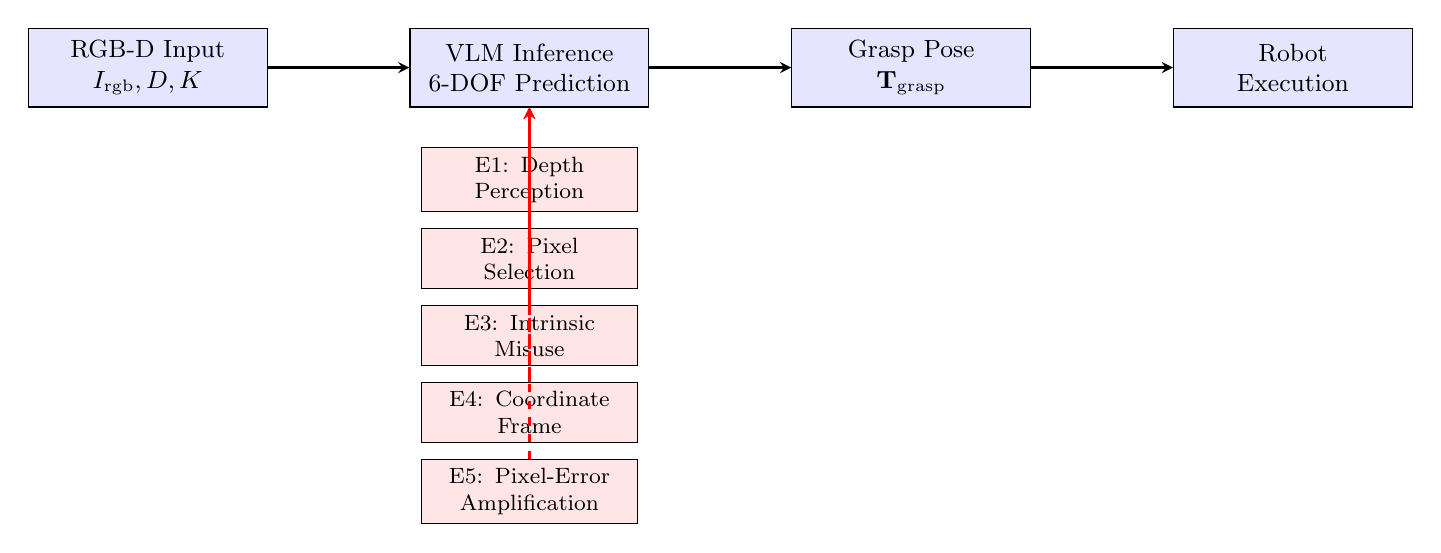
\begin{tikzpicture}[node distance=1.8cm, auto,
    block/.style={rectangle, draw, fill=blue!10, text width=2.8cm, text centered, minimum height=1cm, font=\small},
    error/.style={rectangle, draw, fill=red!10, text width=2.5cm, text centered, minimum height=0.7cm, font=\footnotesize},
    arrow/.style={->, >=stealth, thick}]

    \node [block] (rgbd) {RGB-D Input\\$I_{\text{rgb}}, D, K$};
    \node [block, right=of rgbd] (vlm) {VLM Inference\\6-DOF Prediction};
    \node [block, right=of vlm] (pose) {Grasp Pose\\$\mathbf{T}_{\text{grasp}}$};
    \node [block, right=of pose] (exec) {Robot\\Execution};

    \node [error, below=0.5cm of vlm] (e1) {E1: Depth\\Perception};
    \node [error, below=0.2cm of e1] (e2) {E2: Pixel\\Selection};
    \node [error, below=0.2cm of e2] (e3) {E3: Intrinsic\\Misuse};
    \node [error, below=0.2cm of e3] (e4) {E4: Coordinate\\Frame};
    \node [error, below=0.2cm of e4] (e5) {E5: Pixel-Error\\Amplification};

    \draw [arrow] (rgbd) -- (vlm);
    \draw [arrow] (vlm) -- (pose);
    \draw [arrow] (pose) -- (exec);
    \draw [arrow, red, dashed] (e1) -- (vlm);
    \draw [arrow, red, dashed] (e2) -- (vlm);
    \draw [arrow, red, dashed] (e3) -- (vlm);
    \draw [arrow, red, dashed] (e4) -- (vlm);
    \draw [arrow, red, dashed] (e5) -- (vlm);
\end{tikzpicture}
\caption{Error propagation in VLM-based 6-DOF grasp prediction. Five categories of error (E1--E5) combine to produce inaccurate grasp poses.}
\label{fig:error_flow}
\end{figure}

\subsection{Baseline Performance}

Our current system (semester project) provides two baselines:

\textbf{Baseline A (Option B -- VLM + SAM2 + CGN)}: The VLM outputs 2D grasp region boxes. Depth back-projection and Contact-GraspNet handle all 3D reasoning. The VLM never predicts 3D coordinates. Accuracy is determined by CGN, not the VLM. However, CGN requires a good segmentation mask, and the system is computationally expensive (SAM2 + CGN inference).

\textbf{Baseline B (Option C -- VLM Align)}: The VLM outputs a 2D alignment point and gripper angle. The server samples depth at that point and back-projects to 3D. Position accuracy depends entirely on (a) the VLM choosing the correct pixel and (b) valid depth existing at that pixel. This is lightweight but fragile---no geometric refinement, no collision checking from the VLM side.

\textbf{Baseline C (6-DOF Experiment)}: The VLM receives both RGB and depth-preview (JET) images and is asked to output full 6-DOF coordinates. This is the most ambitious baseline and the one that most directly exhibits the position accuracy problem. Z errors of 2--10~cm (typically 3--8~cm) are observed, making it unsuitable for reliable grasping without further refinement.

% ── 4. Proposed Approach ──────────────────────────────────────────────────
\section{Proposed Approach}

We propose a systematic exploration of four complementary research directions, illustrated in Figure~\ref{fig:directions}. Each direction attacks the position accuracy problem from a different angle, and the directions can be combined.

\begin{figure}[H]
\centering
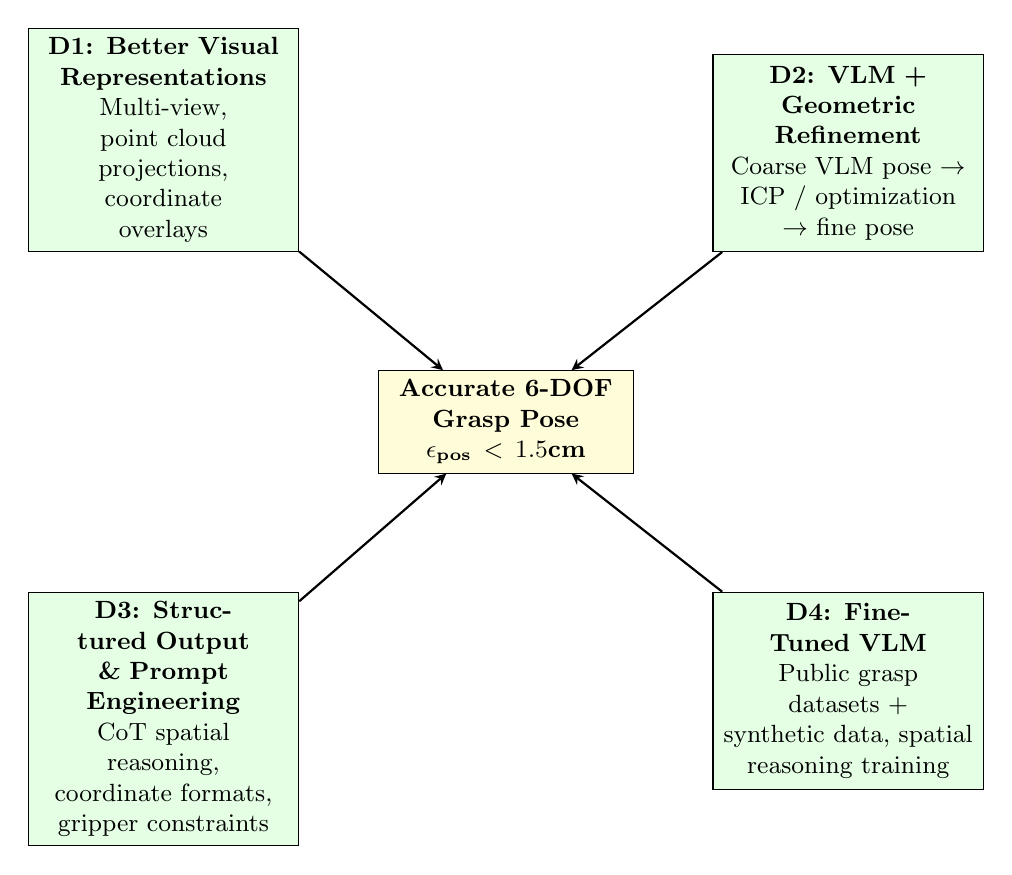
\begin{tikzpicture}[node distance=2cm and 1.5cm, auto,
    dir/.style={rectangle, draw, fill=green!10, text width=3.2cm, text centered, minimum height=2.5cm, font=\small},
    center/.style={rectangle, draw, fill=yellow!15, text width=3cm, text centered, minimum height=1.2cm, font=\small\bfseries}]

    \node [center] (goal) {Accurate 6-DOF\\Grasp Pose\\$\epsilon_{\text{pos}} < 1.5\text{cm}$};

    \node [dir, above left=1.5cm and 1cm of goal] (d1) {\textbf{D1: Better Visual\\Representations}\\Multi-view, point cloud\\projections, coordinate\\overlays};
    \node [dir, above right=1.5cm and 1cm of goal] (d2) {\textbf{D2: VLM + Geometric\\Refinement}\\Coarse VLM pose $\rightarrow$\\ICP / optimization\\$\rightarrow$ fine pose};
    \node [dir, below left=1.5cm and 1cm of goal] (d3) {\textbf{D3: Structured Output\\\& Prompt Engineering}\\CoT spatial reasoning,\\coordinate formats,\\gripper constraints};
    \node [dir, below right=1.5cm and 1cm of goal] (d4) {\textbf{D4: Fine-Tuned VLM}\\Public grasp datasets +\\synthetic data, spatial\\reasoning training};

    \draw [->, >=stealth, thick] (d1) -- (goal);
    \draw [->, >=stealth, thick] (d2) -- (goal);
    \draw [->, >=stealth, thick] (d3) -- (goal);
    \draw [->, >=stealth, thick] (d4) -- (goal);
\end{tikzpicture}
\caption{Four complementary research directions, all targeting the same accuracy goal.}
\label{fig:directions}
\end{figure}

\subsection{Direction 1: Better Visual Representations for 3D-Aware VLM Input}

\textbf{Hypothesis}: The information loss from encoding 3D structure (depth) as a 2D JET colormap is a primary source of VLM position error. Providing richer, more quantitative 3D representations will improve VLM coordinate predictions---consistent with SpatialRGPT~\cite{cheng2024spatialrgpt}, which found that explicitly injecting depth into the visual interface improves spatial reasoning.

\textbf{Approach}: We will systematically compare the following input representations:

\begin{enumerate}[label=\textbf{R\arabic*:}, leftmargin=*]
    \item \textbf{RGB only} (Baseline C): Current 6-DOF experiment baseline. VLM receives RGB + JET depth visualization.
    \item \textbf{RGB + depth as normalized grayscale}: Depth encoded as a single-channel grayscale image with linear mapping (0--2.5~m $\rightarrow$ 0--255). Preserves metric linearity at the cost of perceptual contrast.
    \item \textbf{RGB + annotated keypoint with local depth}: Instead of full depth image, overlay depth values (in mm) as text annotations at key spatial locations (object center, grasp point candidates, table plane). This exploits the VLM's text-reading capability for precise depth communication.
    \item \textbf{RGB + multi-view point cloud projections}: Render the back-projected point cloud from 2--3 canonical viewpoints (top-down, side, front) and provide these as additional images. The VLM sees explicit 3D structure rather than having to reconstruct it from 2D depth.
    \item \textbf{RGB + coordinate grid overlay}: Overlay a sparse grid of $(u, v, Z)$ annotations on the RGB image (every 100 pixels), giving the VLM explicit spatial reference points for interpolation.
    \item \textbf{RGB + surface normal map}: Encode surface orientation as an RGB image where $(R,G,B)$ maps to $(n_x, n_y, n_z)$. Surface normals are viewpoint-invariant and directly indicate graspable surface orientation.
\end{enumerate}

\textbf{Evaluation}: For each representation, we will measure:
\begin{itemize}[nosep]
    \item 3D position error: $\|\mathbf{t}_{\text{pred}} - \mathbf{t}_{\text{gt}}\|$ (Euclidean distance in camera frame).
    \item Depth (Z) error: $|Z_{\text{pred}} - Z_{\text{gt}}|$.
    \item Pixel selection quality: whether the VLM's chosen pixel lands on valid, stable object surface.
    \item Grasp success rate in physical robot trials (for the top 2--3 representations).
\end{itemize}

\textbf{Implementation}: All representations can be generated from the existing \texttt{camera\_data.npy} format. The VLM API calls will be constructed similarly to the existing \texttt{align\_6dof\_experiment.ipynb} pattern, with the multi-image payload adapted for each representation.

\subsection{Direction 2: VLM + Geometric Refinement Pipeline}

\textbf{Hypothesis}: VLMs can provide a useful coarse initialization (within 3--5~cm), which classical geometric optimization can refine to sub-centimeter accuracy. The VLM's semantic understanding complements the optimizer's numerical precision. This coarse-to-fine decomposition follows the pattern validated by CoPa~\cite{huang2024copa}, but we study it systematically across refinement methods and initialization qualities.

\textbf{Approach}: We design a two-stage pipeline:

\begin{enumerate}[leftmargin=*]
    \item \textbf{Stage 1 -- VLM Coarse Prediction}: The VLM outputs an initial 6-DOF grasp pose $\mathbf{T}_{\text{coarse}}$ using the best visual representation from Direction 1. The output includes:
    \begin{itemize}[nosep]
        \item 3D position $\mathbf{t}_{\text{coarse}}$ and orientation (as gripper angle $\theta$).
        \item The 2D pixel $(u, v)$ the prediction is based on.
        \item A confidence estimate.
    \end{itemize}

    \item \textbf{Stage 2 -- Geometric Refinement}: Given $\mathbf{T}_{\text{coarse}}$ and the local point cloud (from back-projected depth within a region around $(u, v)$), apply one or more of:
    \begin{enumerate}[label=\alph*.]
        \item \textbf{ICP (Iterative Closest Point)}: Fit a gripper-scale bounding box or cylinder to the local point cloud, aligning the grasp frame to the local surface geometry.
        \item \textbf{Surface normal alignment}: Use PCA on the local point cloud to estimate the local surface normal and principal curvature directions. Rotate the grasp frame so the approach direction aligns with the surface normal (or a desired offset), and the closing direction aligns with the minor curvature axis.
        \item \textbf{Depth-based position correction}: Sample the raw depth at the VLM's pixel (with 5$\times$5 median filtering) and re-compute the 3D position using the actual intrinsics, overriding the VLM's estimated Z. This is the existing Option C approach --- we evaluate whether it alone is sufficient.
        \item \textbf{Optimization-based refinement}: Formulate grasp quality as an objective function over $\mathbf{T}$ (combining surface alignment, distance to VLM prior, collision avoidance, and grasp width feasibility) and optimize via gradient descent or sampling in $SE(3)$.
    \end{enumerate}
\end{enumerate}

\textbf{Key Research Questions}:
\begin{itemize}[nosep]
    \item At what error threshold does VLM initialization become useless for refinement? (I.e., what is the basin of convergence?)
    \item Which refinement method provides the best accuracy-efficiency trade-off?
    \item Can the VLM provide a meaningful confidence score that indicates when refinement is likely to succeed vs.\ fail?
\end{itemize}

\textbf{Evaluation}: For each refinement method, measure:
\begin{itemize}[nosep]
    \item Final position error after refinement.
    \item Refinement success rate (does it converge or diverge?).
    \item Computation time (target: $<100$~ms for real-time use).
    \item Ablation: performance with and without VLM initialization (compare against purely geometric baselines).
\end{itemize}

\subsection{Direction 3: Structured Output Formats and Prompt Engineering}

\textbf{Hypothesis}: The way we ask the VLM to output 3D coordinates significantly impacts accuracy. Chain-of-thought reasoning, explicit coordinate system grounding, and structured output constraints can reduce errors.

\textbf{Approach}: We will systematically evaluate prompt design choices:

\begin{enumerate}[label=\textbf{P\arabic*:}, leftmargin=*]
    \item \textbf{Coordinate format}: Compare the VLM outputting:
    \begin{itemize}[nosep]
        \item \textbf{Direct 3D}: $[X, Y, Z]$ in meters (current approach --- requires the VLM to do deprojection).
        \item \textbf{Pixel + depth}: $(u, v, Z)$ --- the VLM selects the pixel, estimates Z, but deprojection is done server-side with correct intrinsics. This separates pixel selection error from arithmetic error.
        \item \textbf{Pixel + depth band}: $(u, v, \text{depth\_category})$ where the VLM only categorizes depth into coarse bands, and the server refines.
        \item \textbf{Multiple candidate pixels}: $(u_1, v_1), \ldots, (u_k, v_k)$ with the server evaluating depth validity at each and selecting the best.
    \end{itemize}

    \item \textbf{Spatial chain-of-thought}: Ask the VLM to reason step-by-step:
    \begin{enumerate}[nosep]
        \item Identify the target object and its 3D extent from the depth image.
        \item Locate the graspable part and estimate its approximate 3D center.
        \item Identify a precise grasp point, describing its pixel location relative to visible features.
        \item Estimate the depth at that point by comparing with neighboring depth values.
        \item Verify that the estimated width along the closing direction is within gripper limits.
    \end{enumerate}

    \item \textbf{Explicit coordinate system grounding}: Include a coordinate frame visualization (RGB image with overlaid axes) and explicit reference markers, in the spirit of mark-based visual prompting~\cite{liu2024moka}.

    \item \textbf{Gripper-aware constraints}: Encode the gripper's physical limits (80~mm max opening, 20~mm min opening, approach direction, finger dimensions) as quantitative constraints in the prompt, with pixel-scale conversion at the reference depth.

    \item \textbf{Multi-step dialogue}: Instead of a single prompt, use a 2--3 turn conversation following the iterative visual prompting paradigm of PIVOT~\cite{nasiriany2024pivot}:
    \begin{enumerate}[nosep]
        \item Turn 1: VLM identifies the target object and proposes coarse grasp zones.
        \item Turn 2: Server provides zoomed-in views and precise depth values at proposed points.
        \item Turn 3: VLM outputs final refined 6-DOF coordinates.
    \end{enumerate}
    Each additional VLM round trip costs 1--3~s, so multi-turn variants trade latency for accuracy; they are evaluated against the separate latency budget defined in Section~\ref{sec:success}.
\end{enumerate}

\textbf{Evaluation}: Same metrics as Direction 1 (position error, depth error, pixel quality), with the addition of:
\begin{itemize}[nosep]
    \item Output format compliance rate (does the VLM follow the requested format?).
    \item Arithmetic correctness (when VLM does deprojection, does the math check out?).
    \item Reasoning quality (human evaluation of chain-of-thought coherence).
\end{itemize}

\subsection{Direction 4: Fine-Tuned VLM for Spatial Coordinate Prediction}

\textbf{Hypothesis}: General-purpose VLMs lack training on metric 3D reasoning. Fine-tuning on a targeted dataset of RGB-D images with 6-DOF grasp annotations can teach the model to predict accurate coordinates.

\textbf{Approach}:

\begin{enumerate}[leftmargin=*]
    \item \textbf{Training Data}: Rather than building a synthetic pipeline from scratch, we will primarily leverage existing large-scale public datasets: PRISM~\cite{graspmolmo} (379K task-grasp pairs over 10,000 cluttered scenes) and Grasp-Anything-6D~\cite{lgrasp6d} (1M point-cloud scenes with language-associated grasps), converting their annotations into our RGB-D + camera-frame 6-DOF output format. A smaller complementary self-generated set (PyBullet / Isaac Sim, $\sim$1--5K scenes matched to our tabletop domain, camera intrinsics, and gripper) will be used for domain adaptation and held-out evaluation. This follows the synthetic-data recipes validated by SpatialVLM~\cite{chen2024spatialvlm} and GraspMolmo~\cite{graspmolmo}, and removes the schedule risk of building a data pipeline from scratch.

    \item \textbf{Model Selection}: Fine-tune an open-weight VLM (e.g., Molmo~\cite{deitke2025molmo}, LLaVA, or Qwen2-VL) using LoRA for parameter efficiency---the recipe RoboPoint~\cite{yuan2024robopoint} showed to work for image-space affordance points, here extended from 2D points to metric camera-frame 6-DOF poses. The model receives:
    \begin{itemize}[nosep]
        \item RGB image + depth representation (best format from Direction 1).
        \item Task specification text.
    \end{itemize}
    and outputs 6-DOF grasp coordinates in a structured format.

    \item \textbf{Training Objective}: Multi-task loss combining:
    \begin{itemize}[nosep]
        \item 3D position regression loss: $\mathcal{L}_{\text{pos}} = \|\mathbf{t}_{\text{pred}} - \mathbf{t}_{\text{gt}}\|_2$.
        \item Orientation loss: $\mathcal{L}_{\text{ori}} = \|\mathbf{R}_{\text{pred}} - \mathbf{R}_{\text{gt}}\|_F$ or angular error.
        \item Auxiliary pixel classification loss: cross-entropy on whether each pixel is a valid grasp point.
        \item Standard language modeling loss on chain-of-thought reasoning tokens.
    \end{itemize}

    \item \textbf{Evaluation}: Compare fine-tuned model against:
    \begin{itemize}[nosep]
        \item Zero-shot VLM (same base model, no fine-tuning).
        \item The best prompt-engineered approach from Direction 3.
        \item The Option B pipeline (VLM + SAM2 + CGN) as an upper bound on geometric accuracy.
    \end{itemize}
\end{enumerate}

\textbf{Key Research Questions}:
\begin{itemize}[nosep]
    \item How much training data is needed for meaningful improvement? (W8 pilot at 2 scales, e.g.\ 5K and 50K examples; the full 1K--380K sweep is run only if the pilot shows signal.)
    \item Does fine-tuning for coordinate prediction degrade the VLM's general semantic reasoning?
    \item Can a fine-tuned model generalize to real-world scenes without real-world fine-tuning data? (Sim-to-real transfer.)
    \item Is LoRA sufficient, or is full fine-tuning needed for spatial reasoning?
\end{itemize}

\subsection{Integration and Comparative Evaluation}

The four directions are not mutually exclusive. After individual evaluation, we will test the most promising combinations:

\begin{itemize}[nosep]
    \item D1 (best representation) + D2 (geometric refinement): Does better input representation improve the coarse initialization enough to guarantee refinement convergence?
    \item D1 (best representation) + D3 (best prompt): Do better inputs and better prompting compound or saturate?
    \item D1 + D3 + D4 (fine-tuning with best representation and prompt format): Does the fine-tuned model benefit from representation and prompt optimizations discovered in the zero-shot setting?
    \item D1 + D2 + D3: The full zero-shot pipeline.
\end{itemize}

Table~\ref{tab:experiments} summarizes the planned experimental matrix.

\begin{table}[H]
\centering
\caption{Planned experimental matrix. Each cell represents a set of experiments.}
\label{tab:experiments}
\begin{tabular}{@{}lcccc@{}}
\toprule
& \textbf{D1 (Repr.)} & \textbf{D2 (Refine.)} & \textbf{D3 (Prompt)} & \textbf{D4 (FT)} \\
\midrule
Phase 1 (individual) & 6 variants & 4 methods & 5 formats & 2 scales (pilot) \\
Phase 2 (combined) & \multicolumn{4}{c}{Best D1 + Best D2, Best D1 + Best D3, D1+D2+D3, D1+D3+D4} \\
Phase 3 (robot)  & \multicolumn{4}{c}{Top 3 pipelines on physical robot (20 trials each, 3 objects)} \\
\bottomrule
\end{tabular}
\end{table}

% ── 5. Methodology ────────────────────────────────────────────────────────
\section{Methodology}

\subsection{Data}
\label{sec:data}

\textbf{Real-World Data}: We will use the existing 13 capture sequences from the semester project (\texttt{rgbd\_data/captures/}), plus $\sim$30--50 new captures with varied objects (cups, bottles, tools, boxes), clutter levels, and lighting conditions. Each capture contains:
\begin{itemize}[nosep]
    \item \texttt{camera\_data.npy}: RGB (1280$\times$720), depth (float32, meters), intrinsics K.
    \item Depth from RealSense D455 active stereo (specified $<$2\% error at 4~m; typically a few mm at our 0.5--1~m working distance), which is accurate enough to resolve the 1--1.5~cm target.
\end{itemize}

\textbf{Ground-Truth Grasps}: Since manual 6-DOF annotation is impractical, we will use:
\begin{itemize}[nosep]
    \item Contact-GraspNet on manually verified segmentation masks to generate a \emph{set} of reference grasps $\mathcal{G}^* = \{\mathbf{T}^*_1, \ldots, \mathbf{T}^*_m\}$ per target part (all candidates above a quality threshold), rather than a single pseudo-ground-truth pose. Using a set avoids penalizing predictions that are valid but differ from one arbitrary reference grasp.
    \item Human evaluation: for each prediction, a human annotator rates grasp quality (1--5) based on the RGB-D visualization.
    \item Physical trial success/failure as the ultimate ground truth in Phase 3.
\end{itemize}

\subsection{Evaluation Metrics}

\begin{enumerate}[label=\textbf{M\arabic*:}, leftmargin=*]
    \item \textbf{3D Position Error}: $\epsilon_{\text{pos}} = \min_{\mathbf{T}^* \in \mathcal{G}^*} \|\mathbf{t}_{\text{pred}} - \mathbf{t}^*\|_2$ (cm), i.e.\ distance to the \emph{nearest} reference grasp. Primary metric; we additionally report success-at-threshold curves $\Pr[\epsilon_{\text{pos}} < \delta]$ for $\delta \in [0.5, 3]$~cm rather than a single cutoff.
    \item \textbf{Depth (Z) Error}: $\epsilon_Z = |Z_{\text{pred}} - Z_{\text{gt}}|$ (cm), where $Z_{\text{gt}}$ is the median-filtered sensor depth at the reference pixel. Isolates depth perception from lateral error.
    \item \textbf{Lateral Error}: $\epsilon_{XY} = \sqrt{(X_{\text{pred}} - X_{\text{gt}})^2 + (Y_{\text{pred}} - Y_{\text{gt}})^2}$ (cm), against the nearest reference grasp.
    \item \textbf{Orientation Error}: geodesic rotation error $\epsilon_R = \min_{\mathbf{T}^* \in \mathcal{G}^*} \arccos\big(\tfrac{1}{2}(\mathrm{tr}(\mathbf{R}_{\text{pred}}^\top \mathbf{R}^*) - 1)\big)$ (degrees), taking the minimum over the object's symmetry group for symmetric objects. The in-plane gripper angle error $\epsilon_{\theta} = |\theta_{\text{pred}} - \theta_{\text{gt}}|$ is reported separately as a diagnostic.
    \item \textbf{Pixel Selection Validity}: Binary --- does the VLM's chosen pixel have valid depth (finite, $>$0) within a 5$\times$5 window?
    \item \textbf{Pixel Selection Quality}: Distance from chosen pixel to the nearest ``good'' grasp pixel (manually annotated for a subset).
    \item \textbf{Grasp Success Rate}: Physical robot trial success (object lifted, held for 3 seconds, no collision). Phase 3 only.
    \item \textbf{Inference Time}: Wall-clock time from image capture to grasp pose output (ms).
\end{enumerate}

\textbf{Statistical Protocol}: VLM outputs are stochastic. All API calls use temperature 0 where supported; each (scene, method) pair is queried $N=3$ times and we report mean $\pm$ standard deviation. Because every method is evaluated on the same capture set, method comparisons (across representations, refinement methods, and prompt formats) use paired tests (Wilcoxon signed-rank, $\alpha = 0.05$).

\subsection{Baselines}

\begin{enumerate}[leftmargin=*]
    \item \textbf{Option B (VLM + SAM2 + CGN)}: The full geometric pipeline. Represents the current best accuracy at the cost of complexity.
    \item \textbf{Option C (VLM 2D Align)}: VLM returns 2D point; server back-projects. Represents the simplest VLM-based approach.
    \item \textbf{6-DOF VLM (Baseline C)}: VLM receives RGB + JET depth, outputs full 6-DOF. Current direct prediction baseline.
    \item \textbf{Geometric-only}: CGN on full-scene point cloud without VLM guidance. Measures the value added by VLM semantic reasoning.
    \item \textbf{Random + Refinement}: Random pose initialization + geometric refinement. Tests whether refinement alone can solve the problem without semantic initialization.
\end{enumerate}

\subsection{Hardware and Software}

\begin{itemize}[nosep]
    \item \textbf{Camera}: Intel RealSense D455 (1280$\times$720 RGB-D, aligned depth).
    \item \textbf{Robot}: Franka Emika Panda (7-DOF) with parallel-jaw gripper (80~mm max opening).
    \item \textbf{VLM APIs}: Gemini (\texttt{gemini-robotics-er-1.6-preview}~\cite{gemini2025robotics}), OpenAI (GPT-4o), plus open-weight models~\cite{deitke2025molmo} for fine-tuning.
    \item \textbf{Compute}: Local workstation with NVIDIA GPU for SAM2, CGN, and fine-tuning.
    \item \textbf{Software}: Existing \texttt{vla-grasp-server} codebase + ROS2 + Pinocchio IK solver.
\end{itemize}

% ── 6. Expected Outcomes ──────────────────────────────────────────────────
\section{Expected Outcomes and Contributions}

\subsection{Primary Expected Results}

\begin{enumerate}[leftmargin=*]
    \item \textbf{Error source quantification}: A detailed breakdown of how much each error category (E1--E5) contributes to overall position inaccuracy, informing future research priorities.

    \item \textbf{Representation guidelines}: Evidence-based recommendations for how to encode 3D information for VLM consumption. Expected finding: grayscale depth with text annotations outperforms JET colormap for metric prediction tasks.

    \item \textbf{Refinement recipe}: A validated coarse-to-fine pipeline where VLM semantic initialization + geometric refinement achieves sub-centimeter accuracy. Expected finding: ICP or surface normal alignment with VLM initialization within 3~cm converges reliably.

    \item \textbf{Prompt design principles}: Guidelines for structured VLM output formats that improve spatial reasoning. Expected finding: separating pixel selection (VLM strength) from deprojection math (server strength) yields the best accuracy.

    \item \textbf{Fine-tuning feasibility}: A pilot assessment of whether LoRA fine-tuning on existing public grasp datasets (PRISM, Grasp-Anything-6D) can meaningfully improve VLM 3D coordinate prediction, and at what data scale.
\end{enumerate}

\subsection{Engineering Contributions}

\begin{enumerate}[leftmargin=*]
    \item Extended \texttt{vla-grasp-server} with pluggable 6-DOF prediction backends, enabling rapid A/B testing of new approaches.
    \item A standardized evaluation harness for VLM grasp pose prediction with automated metrics computation.
    \item A synthetic data generation pipeline for grasp pose training data.
    \item Public release of all prompts, evaluation data, and (if successful) fine-tuned model weights.
\end{enumerate}

\subsection{Success Criteria}
\label{sec:success}

The project will be considered successful if:
\begin{enumerate}[nosep]
    \item At least one proposed method achieves $\epsilon_{\text{pos}} < 1.5$~cm on $\geq$80\% of test captures. The 1.5~cm threshold is derived from the lateral tolerance of the 80~mm parallel-jaw gripper on typical 40--60~mm household objects; 1~cm remains the aspirational target.
    \item The best method is integrated into the \texttt{vla-grasp-server} pipeline and runs end-to-end in $<2$ seconds for single-turn pipelines. Multi-turn variants (Direction 3, P5) are evaluated against a separate $<6$~second budget, since each additional VLM round trip costs 1--3~s.
    \item Physical robot trials demonstrate $\geq$70\% grasp success rate on a set of 3 novel objects.
\end{enumerate}

% ── 8. Conclusion ─────────────────────────────────────────────────────────
\section{Conclusion}

This proposal outlines a systematic research plan to address a critical bottleneck in VLM-based robotic grasping: the inability of current VLMs to accurately predict 3D positions and 6-DOF grasp coordinates. By exploring four complementary directions---better visual representations, geometric refinement pipelines, prompt engineering, and model fine-tuning---we aim to reduce 3D position error from the current 2--10~cm to the 1--1.5~cm level, making direct VLM 6-DOF prediction viable for real-world robotic execution.

The work builds directly on the completed semester project \texttt{vla-grasp-server}, leveraging its existing capture pipeline, VLM integration, SAM2 segmentation, Contact-GraspNet inference, and ROS2 execution framework. The proposed experiments are designed to produce actionable insights regardless of which direction proves most successful, and the modular evaluation framework will enable rapid iteration as new VLMs and techniques emerge.

% ── References ────────────────────────────────────────────────────────────
\begin{thebibliography}{99}

\bibitem{sundermeyer2021contact}
M.~Sundermeyer, A.~Mousavian, R.~Triebel, and D.~Fox,
``Contact-GraspNet: Efficient 6-DoF Grasp Generation in Cluttered Scenes,''
in \emph{IEEE International Conference on Robotics and Automation (ICRA)}, 2021.

\bibitem{fang2023anygrasp}
H.-S.~Fang, C.~Wang, H.~Fang, M.~Gou, J.~Liu, H.~Yan, W.~Liu, Y.~Xie, and C.~Lu,
``AnyGrasp: Robust and Efficient Grasp Perception in Spatial and Temporal Domains,''
\emph{IEEE Transactions on Robotics}, vol.~39, no.~5, 2023.

\bibitem{anypart2024}
T.~van~Oort, D.~Miller, W.~N.~Browne, N.~Marticorena, J.~Haviland, and N.~Suenderhauf,
``Open-Vocabulary Part-Based Grasping,''
\emph{arXiv preprint} arXiv:2406.05951, 2024.

\bibitem{affordgrasp}
Y.~Tang, S.~Zhang, X.~Hao, P.~Wang, J.~Wu, Z.~Wang, and S.~Zhang,
``AffordGrasp: In-Context Affordance Reasoning for Open-Vocabulary Task-Oriented Grasping in Clutter,''
in \emph{IEEE/RSJ International Conference on Intelligent Robots and Systems (IROS)}, 2025.

\bibitem{graspcot}
X.~Chu, J.~Deng, G.~You, W.~Liu, X.~Li, J.~Ji, and Y.~Zhang,
``GraspCoT: Integrating Physical Property Reasoning for 6-DoF Grasping under Flexible Language Instructions,''
in \emph{IEEE/CVF International Conference on Computer Vision (ICCV)}, 2025.

\bibitem{graspmolmo}
A.~Deshpande, Y.~Deng, A.~Ray, J.~Salvador, W.~Han, J.~Duan, K.-H.~Zeng, Y.~Zhu, R.~Krishna, and R.~Hendrix,
``GraspMolmo: Generalizable Task-Oriented Grasping via Large-Scale Synthetic Data Generation,''
in \emph{Conference on Robot Learning (CoRL)}, 2025.

\bibitem{lgrasp6d}
T.~Nguyen, M.~N.~Vu, B.~Huang, A.~Vuong, Q.~Vuong, N.~Le, T.~Vo, and A.~Nguyen,
``Language-Driven 6-DoF Grasp Detection Using Negative Prompt Guidance,''
in \emph{European Conference on Computer Vision (ECCV)}, 2024.

\bibitem{graspgenx}
B.~Han, Y.-W.~Chao, E.~Coumans, C.~Eppner, B.~Sundaralingam, J.~Deng, S.~Birchfield, and A.~Murali,
``GraspGen-X: Cross-Embodiment 6-DOF Diffusion-based Grasping,''
in \emph{IEEE/CVF Conference on Computer Vision and Pattern Recognition (CVPR)}, 2026.

\bibitem{activepose}
S.~Liu, Z.~Li, W.~Wang, H.~Sun, H.~Zhang, H.~Chen, Y.~Qin, A.~Ajoudani, and Y.~Wang,
``ActivePose: Active 6D Object Pose Estimation and Tracking for Robotic Manipulation,''
\emph{arXiv preprint} arXiv:2509.11364, 2025.

\bibitem{open6dor}
Y.~Ding, H.~Geng, C.~Xu, X.~Fang, J.~Zhang, S.~Wei, Q.~Dai, Z.~Zhang, and H.~Wang,
``Open6DOR: Benchmarking Open-instruction 6-DoF Object Rearrangement and A VLM-based Approach,''
in \emph{IEEE/RSJ International Conference on Intelligent Robots and Systems (IROS)}, 2024.

\bibitem{oasis}
X.~Chen, S.~Ren, L.~Huang, H.~Sun, M.~Li, X.~Chen, Z.~Liu, and X.~Lan,
``OASIS: Observation-Action Space Alignment via SE(3) Trajectory Prediction for Robotic Manipulation,''
\emph{arXiv preprint} arXiv:2605.25829, 2026.

\bibitem{horyon}
J.~Corsetti, D.~Boscaini, F.~Giuliari, C.~Oh, A.~Cavallaro, and F.~Poiesi,
``High-Resolution Open-Vocabulary Object 6D Pose Estimation,''
\emph{IEEE Transactions on Pattern Analysis and Machine Intelligence}, 2025.

\bibitem{ficop}
Y.~Qin, S.~Fan, F.~Yang, Z.~Xue, Z.~Mai, W.~Chen, K.~Yang, and Z.~Li,
``Learning Fine-Grained Correspondence with Cross-Perspective Perception for Open-Vocabulary 6D Object Pose Estimation,''
\emph{IEEE Robotics and Automation Letters}, 2026.

\bibitem{freegrasp}
R.~Jiao, A.~Fasoli, F.~Giuliari, M.~Bortolon, S.~Povoli, G.~Mei, Y.~Wang, and F.~Poiesi,
``Free-form Language-based Robotic Reasoning and Grasping,''
in \emph{IEEE/RSJ International Conference on Intelligent Robots and Systems (IROS)}, 2025.

\bibitem{hiragrasp}
Y.~Liu, Y.~Hu, Y.~Liu, and M.~Zhong,
``Hi-RAGrasp: A Human-in-the-Loop Experience-Augmented Method for Task-Oriented Grasping,''
\emph{Sensors}, vol.~26, no.~10, art.~no.~3221, 2026.

\bibitem{visograsp}
Y.~Shi, D.~Wen, G.~Chen, E.~Welte, S.~Liu, K.~Peng, R.~Stiefelhagen, and R.~Rayyes,
``VISO-Grasp: Vision-Language Informed Spatial Object-centric 6-DoF Active View Planning and Grasping in Clutter and Invisibility,''
in \emph{IEEE/RSJ International Conference on Intelligent Robots and Systems (IROS)}, 2025.

\bibitem{zhen2024threedvla}
H.~Zhen, X.~Qiu, P.~Chen, J.~Yang, X.~Yan, Y.~Du, Y.~Hong, and C.~Gan,
``3D-VLA: A 3D Vision-Language-Action Generative World Model,''
in \emph{International Conference on Machine Learning (ICML)}, 2024.

\bibitem{yuan2024robopoint}
W.~Yuan, J.~Duan, V.~Blukis, W.~Pumacay, R.~Krishna, A.~Murali, A.~Mousavian, and D.~Fox,
``RoboPoint: A Vision-Language Model for Spatial Affordance Prediction for Robotics,''
in \emph{Conference on Robot Learning (CoRL)}, 2024.

\bibitem{chen2024spatialvlm}
B.~Chen, Z.~Xu, S.~Kirmani, B.~Ichter, D.~Driess, P.~Florence, D.~Sadigh, L.~Guibas, and F.~Xia,
``SpatialVLM: Endowing Vision-Language Models with Spatial Reasoning Capabilities,''
in \emph{IEEE/CVF Conference on Computer Vision and Pattern Recognition (CVPR)}, 2024.

\bibitem{cheng2024spatialrgpt}
A.-C.~Cheng, H.~Yin, Y.~Fu, Q.~Guo, R.~Yang, J.~Kautz, X.~Wang, and S.~Liu,
``SpatialRGPT: Grounded Spatial Reasoning in Vision-Language Models,''
in \emph{Advances in Neural Information Processing Systems (NeurIPS)}, 2024.

\bibitem{deitke2025molmo}
M.~Deitke, C.~Clark, S.~Lee, \emph{et al.},
``Molmo and PixMo: Open Weights and Open Data for State-of-the-Art Vision-Language Models,''
in \emph{IEEE/CVF Conference on Computer Vision and Pattern Recognition (CVPR)}, 2025.

\bibitem{liu2024moka}
F.~Liu, K.~Fang, P.~Abbeel, and S.~Levine,
``MOKA: Open-World Robotic Manipulation through Mark-Based Visual Prompting,''
in \emph{Robotics: Science and Systems (RSS)}, 2024.

\bibitem{nasiriany2024pivot}
S.~Nasiriany, F.~Xia, W.~Yu, T.~Xiao, J.~Liang, \emph{et al.},
``PIVOT: Iterative Visual Prompting Elicits Actionable Knowledge for VLMs,''
in \emph{International Conference on Machine Learning (ICML)}, 2024.

\bibitem{huang2024copa}
H.~Huang, F.~Lin, Y.~Hu, S.~Wang, and Y.~Gao,
``CoPa: General Robotic Manipulation through Spatial Constraints of Parts with Foundation Models,''
in \emph{IEEE/RSJ International Conference on Intelligent Robots and Systems (IROS)}, 2024.

\bibitem{qian2024thinkgrasp}
Y.~Qian, X.~Zhu, O.~Biza, S.~Jiang, L.~Zhao, H.~Huang, Y.~Qi, and R.~Platt,
``ThinkGrasp: A Vision-Language System for Strategic Part Grasping in Clutter,''
in \emph{Conference on Robot Learning (CoRL)}, 2024.

\bibitem{gemini2025robotics}
Gemini Robotics Team, Google DeepMind,
``Gemini Robotics: Bringing AI into the Physical World,''
\emph{arXiv preprint} arXiv:2503.20020, 2025.

\end{thebibliography}

\end{document}
